%% 歩容パターンの再評価手法の提案.tex
%% LaTeX-2e 専用

%% 全体の流れとしては,まず,先行研究の問題点を指摘し,次に,歩容パターンの再評価手法を提案する.

\chapter{歩容パターンの再評価手法の提案}\label{chapter:歩容パターンの再評価手法の提案}
第\ref{chapter:歩容パターンの再評価手法の提案}章では,先行研究の手法およびその問題点を指摘し,
常に脚軌道生成が可能な自由歩容パターン生成手法として,歩容パターンの再評価手法を述べる.

% 先行研究の章
\section{本研究室における自由歩容パターン生成の先行研究}
最初にグラフ探索よる自由歩容パターン生成手法において用いる用語を定義し,
先行研究で行われてきた自由歩容パターン生成手法について述べる.
また,先行研究で用いられてきた自由歩容パターン生成手法の問題点について述べる.

\subsection{グラフ理論について}
本論文ではグラフ理論を用いた自由歩容パターン生成手法を論ずるため,まずはグラフ理論について説明をする.
グラフとは,頂点(ノード)とそれらを結ぶ辺(エッジ)からなる図形である.
このグラフを用いて,さまざまな問題を取り扱う学問をグラフ理論という.

以降の説明を簡単にするため,この論文で用いるグラフ理論の用語について簡潔に述べる.
エッジに向きがあるものを有向グラフ,逆に向きを持たないものを無向グラフという.
また,閉路を持たず,かつ,すべての頂点間に経路が存在するグラフを木という.
このような木構造をもつグラフのうち,図\ref*{fig:tree_graph}のように,
根となるノードを持ち,そのノードからすべてのノードに到達可能なものを根付き木という.

根付き木において,あるノードから遷移可能なノードをそのノードの子ノードと呼ぶ.
逆に,あるノードに遷移可能なノードをそのノードの親ノードと呼ぶ.
親ノードを持たないノードを根ノードと呼び,子ノードを持たないノードを葉ノードと呼ぶ.
また,あるノードから根ノードまでのエッジの数をそのノードの深さと呼び,
根ノード自身の深さは0となる.

図\ref*{fig:tree_graph}においては,ノードAが根ノードであり,ノードB,Cがその子ノードである.
また,ノードB,ノードD,E,ノードCはノードFを子ノードとして持ち,ノードD,E,Fは葉ノードである.
ノードAの深さは0であり,ノードB,Cの深さは1,ノードD,E,Fの深さは2となる.

グラフのあるノードから別のノードに到達するための経路をパスと呼び,
これを求めることをグラフ探索と呼ぶ.
グラフ探索には,深さ優先探索,幅優先探索などのさまざまなアルゴリズムが存在する.
深さ優先探索では,始点となるノードから,深さが深くなる方向を優先して探索を行う.
これに対して,幅優先探索では,始点となるノードから,深さが浅いノードを優先して探索を行う手法である.

\begin{figure}[htbp]
  \begin{center}
    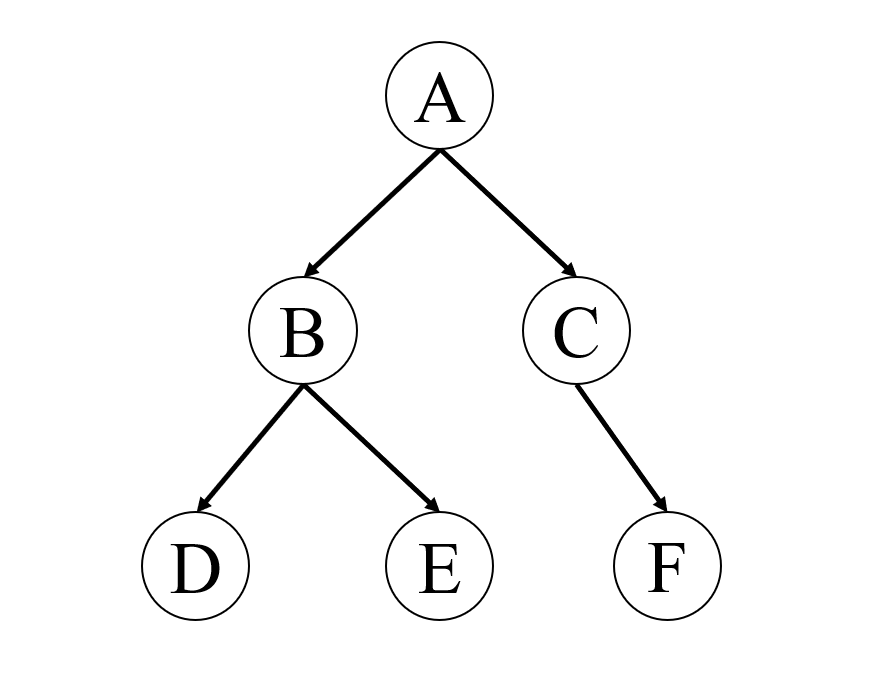
\includegraphics[width=50mm, clip]{figure/tree_graph.png}
   \caption{Tree Graph}
   \label{fig:tree_graph}
  \end{center}
\end{figure}

\subsection{歩容パターングラフの定義}
本研究においては,6脚ロボットの歩容パターンをグラフを用いて表現する.
グラフはロボットの状態をノードとし,ロボットの状態間の遷移,つまりロボットの動作をエッジとして作成する.
グラフは有向の根付き木とし,現在のロボットの状態を根ノード,その姿勢から1動作で到達できる姿勢を子ノードとして根ノードに接続する.
また,このようにして作られたグラフを歩容パターングラフと定義する.

グラフ探索による歩容パターン生成においては,網羅的にロボットの状態を調べ上げるため,
実時間内の計算を行うにはグラフの規模を小さくすることが求められる.
しかし,歩容パターングラフはロボットの状態や動作を対象とするため無数の組み合わせが存在し,
そのすべてを網羅的に調べ上げることは困難である.
そのため,状態や動作を離散化することで歩容パターン生成をグラフへ落とし込む必要がある.
以下に各要素の離散化について述べる.

\subsubsection{グラフの階層構造}
前述のとおり,ロボットの脚位置は脚の可動範囲内であれば,無数の位置を取ることができる.
そのため本手法では,基準となる脚位置を決め,その基準からの相対位置を用いて脚位置を離散化している.
Prabirらが提案した手法では2次元平面での移動を前提としていたが\cite{Prabir_Graph_search},これを三浦が3次元空間へ拡張した\cite{Miura_Graph_search}.

図\ref*{fig:discretization}に支持脚の脚位置の離散化の様子を示した.
図\ref*{fig:discretization}のように脚位置の基準座標を4とし,
脚位置4と同じ高さにあるかつ,進行方向に対して基準位置よりも前方にある脚位置を6,後方にある脚位置を2とする.
また,脚位置6よりも高い位置にある脚位置を7,低い位置にある脚位置を5とし,
脚位置2よりも高い位置にある脚位置を3,低い位置にある脚位置を1とする.
このようにして,脚位置を7つに離散化している.
遊脚している脚の脚位置は,支持脚の脚位置1$\sim$7に対応させ,脚位置1'$\sim$7'とする.% $\sim$ で波線を引く

これにより,脚位置1$\sim$7から脚位置1'$\sim$7'への遷移によって,脚の遊脚運動を表現することができる.
同様に,脚位置1$\sim$7から脚位置1$\sim$7への遷移によって,脚の接地運動を表現することができる.
また,脚位置1'$\sim$7'内での遷移によって,脚の前後移動を表現することができる.
以上より,脚の水平方向の移動と垂直方向の移動をグラフで表現することができることを示した.

\begin{figure}[htbp]
  \begin{center}
   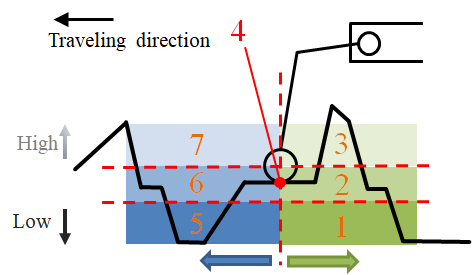
\includegraphics[width=75mm, clip]{figure/chapter2/discretization_of_leg_pos.png}
   \caption{Discretization of Leg Posistion}
   \label{fig:discretization}
  \end{center}
\end{figure}

このような脚位置の離散化を行うことで,脚位置の組み合わせを有限個に抑えることができるが,
脚位置の組み合わせは,$7^6 = 117649$通り存在する.C++では約1秒間に$10^8$回の計算が可能であるため,
この組み合わせの数では実時間内の計算が困難である.
そこで,大木らは脚位置の組み合わせを階層構造化することで探索するノード数を減らすことに成功した\cite{Oki_Graph_search}.

\begin{equation}
    7^6 = 117649
\end{equation}



\begin{figure}[htbp]
  \begin{center}
    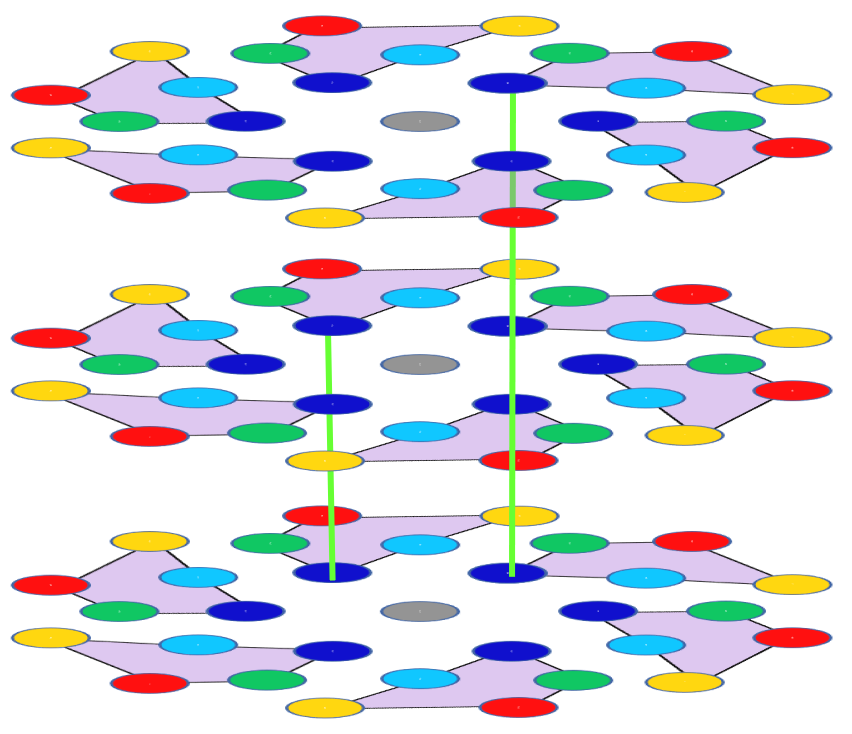
\includegraphics[width=75mm, clip]{figure/chapter2/hierarchy.png}
   \caption{Discretization of Leg Posistion}
   \label{fig:hierarchy}
  \end{center}
\end{figure}

\begin{figure}[htbp]
  \begin{center}
    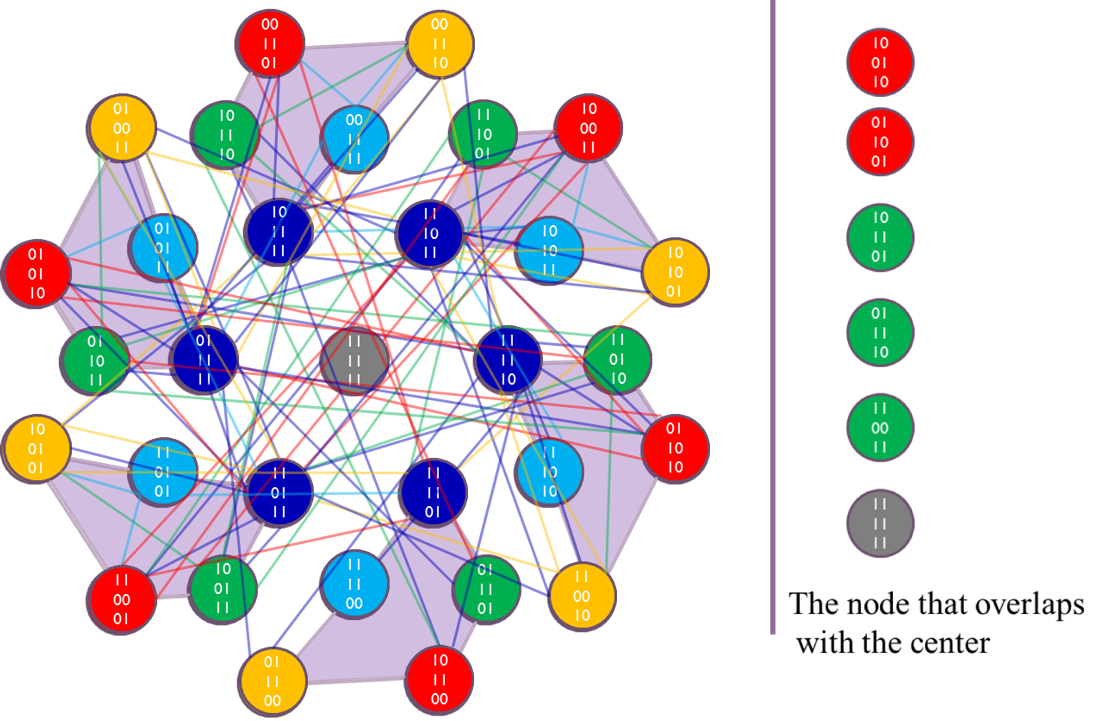
\includegraphics[width=75mm, clip]{figure/chapter2/hierarchy2.png}
   \caption{Discretization of Leg Posistion}
   \label{fig:hierarchy2}
  \end{center}
\end{figure}

\subsubsection{脚軌道生成の分離}
次に歩容パターングラフのエッジの定義について述べる.
歩容パターングラフにおいて,エッジはロボットの動作を表す.
ロボットの動作は脚の接地・遊脚運動と,重心の移動からなるため,これらの動作に対応するエッジを作成する.
具体的には,脚の上下移動のエッジ,脚の水平移動のエッジ,重心の上下移動のエッジ,
重心の水平移動のエッジ,そして,重心の回転のエッジを用いてロボットの動作を表現する.

これらのエッジには,移動前と移動後のノードを補完するための状態を持っておらず,単純に移動前と移動後のノードを結ぶのみである.
これはつまり,歩容パターングラフを生成するプログラムと,脚軌道を生成するプログラムが分離されていることを意味する.
脚軌道を考える場合,ロボットの関節の可動範囲を考慮する必要があり,逆運動学解を用いて脚の関節角度の計算が求められる.
しかし,逆運動学の計算には計算負荷の大きい逆三角関数の計算が必要となり,各エッジについて網羅的に計算を行うことを考えると,
実時間内の計算が困難になってしまう.
そのため本手法では,歩容パターングラフを生成するプログラムを分離し,
歩容パターングラフの生成時には脚の可動範囲は近似的な値を用いて計算することで,
実時間内の計算を可能にしている.

近似的な脚の可動範囲については,以下の手順を用いて求めている.

\subsection{脚軌道生成の失敗}


% 予備実験の章
\section{歩行シミュレーションによる脚軌道生成失敗時の脚先位置の特定}

\subsection{シミュレーション実験の目的}
先行研究では脚軌道生成の失敗による動作の停止が報告された上,その原因は脚先が脚の可動範囲の外を通ることによるものであると考察されてきた.
しかし,具体的に脚先がどのような位置になると脚軌道生成が失敗するのかは明らかにされていなかった.
そのため予備実験として,先行研究と同じ条件で歩行シミュレーション実験を行い,ロボットの脚軌道を確認することで,脚軌道生成失敗の原因を考察した.

\subsection{シミュレーションの条件}
本研究室ではロボットの動作のシミュレーションを行うためのシミュレーターソフトウェアを自作し,シミュレーション実験で用いてきた.
シミュレーターはC++で記述されており,WindowsAPIを用いてGUIを実装し,ロボットを表示している.
また,GUIの表示のプログラムをより簡単に記述するため,ゲームプログラミングに用いられるライブラリのDxLibを用いている.

シミュレーターは物理演算を行っておらず,トルク不足や摩擦,脚先の滑りによるずれを考慮していない.
そのため,ロボットのアクチュエータは無限のトルクを持ち,脚先は滑りなく接地するものと仮定している.
本来これらのパラメータを考慮すべきではあるが,
本研究においては歩容パターン生成によって得られた脚接地点に脚先を届かせることが可能であるかを確認することが目的であるため,これらのパラメータは考慮しないこととしている.

\subsection{シミュレーションの結果}
以下の図に脚軌道生成失敗時の脚先の座標を示す.

\subsection{脚軌道生成の失敗の原因の考察}

% 常に脚軌道生成が可能な自由歩容パターン生成手法の検討の章
\section{常に脚軌道生成が可能な自由歩容パターン生成手法の検討}
常に脚軌道生成を可能にするためには,近似された脚可動範囲を適切に設定する必要がある.


\section{歩容パターンの再評価手法}

